\documentclass[final]{agujournal2019}
\usepackage{apacite}
\usepackage{booktabs}
\usepackage{amsmath}
\usepackage{url}

\journalname{Water Resources Research}

\begin{document}

\title{Attack-Method Choice Changes Robustness Conclusions for a Standard LSTM Rainfall-Runoff Model}

\authors{
Y.~Sun\affil{1}
}
\affiliation{1}{College of Hydrology and Water Resources, Hohai University, Nanjing, China}

\correspondingauthor{Y.~Sun}{sunyiq@hhu.edu.cn}

\begin{keypoints}
\item Iterative adversarial perturbations (Auto-PGD) reveal 17.5$\times$ greater median vulnerability than Gaussian random noise for a 531-basin CAMELS-US benchmark LSTM at $\varepsilon = 0.1$.
\item NSE-based headline statistics use 514 finite basin metrics; one-third of these basins fall below NSE $= 0$ under iterative attack at observation-error-scale perturbation budgets.
\item Statistically undetectable perturbations that preserve input-feature means and standard deviations still cause substantial degradation, indicating that routine quality control is insufficient.
\end{keypoints}

\begin{abstract}
Deep learning models, particularly Long Short-Term Memory (LSTM) networks, have demonstrated strong predictive skill in rainfall-runoff modeling. As these models move toward operational deployment, their robustness to input uncertainty becomes a critical concern. Yet existing assessments often rely on random noise or single-step adversarial methods (FGSM), which may underestimate worst-case vulnerability. Here we present a multi-level adversarial stress test of a 531-basin CAMELS-US temporal benchmark LSTM, employing a spectrum of perturbation methods from random noise through iterative optimization (Auto-PGD), three constraint levels of increasing plausibility, and targeted attacks on flood and pre-event windows. These perturbations are not intended to reproduce the empirical distribution of real-world forcing errors; rather, they serve as constrained worst-case stress tests within observation-error-scale uncertainty budgets. We find that this model is substantially more fragile than random-noise testing suggests: at $\varepsilon = 0.1$, Auto-PGD causes a median NSE degradation of 0.41 across 514 finite basin metrics, compared to 0.02 for Gaussian noise, an adversarial-to-random ratio of 17.5:1. FGSM gives a similar but weaker median degradation of 0.36, indicating that the largest conclusion change is between random and gradient-based testing, while iterative optimization still strengthens the attack. Under Auto-PGD, 167 of 514 finite basins (32.5\%) fall below NSE $= 0$. Furthermore, perturbations that preserve the statistical properties of input features (mean and standard deviation) still cause significant degradation (median $\Delta$NSE $= -0.19$), suggesting that standard quality-control procedures cannot detect all harmful input-error patterns. These results show that robustness assessment for standard hydrological deep-learning configurations requires multi-level stress testing: random-noise sensitivity analysis substantially underestimates the vulnerability that gradient-based adversarial attacks reveal.
\end{abstract}

\section*{Plain Language Summary}
LSTM neural networks are increasingly used for streamflow prediction and are moving toward operational use. We tested how sensitive a standard 531-basin CAMELS-US benchmark LSTM rainfall-runoff model is to small but structured errors in its weather inputs within realistic uncertainty bounds. Using an optimization method called Auto-PGD, we searched for the most harmful input errors allowed by those bounds. These perturbations are not meant to mimic the most common real-world errors; they are stress tests that ask how badly the model can fail if the input errors happen to align with its sensitivities. Across 514 basins with finite NSE metrics, these constrained worst-case perturbations were about 17.5 times more damaging than Gaussian random noise of the same magnitude. The commonly used FGSM attack found much of the same vulnerability at $\varepsilon=0.1$, but remained weaker than iterative Auto-PGD, especially at larger perturbation budgets. Nearly one in three finite basins fell below NSE $=0$ under iterative attack. We also found that some harmful perturbations would pass standard data-quality checks because they preserve the mean and standard deviation of the input variables. These results do not imply that all LSTM models should not be deployed, but they show that standard hydrological deep-learning configurations need stronger stress testing than random-noise sensitivity analysis alone.

%% ====================================================================
\section{Introduction}
%% ====================================================================

Long Short-Term Memory (LSTM) networks have transformed hydrological prediction over the past decade. Beginning with the pioneering work of \citeA{Kratzert2018}, deep learning models have consistently matched or exceeded the performance of process-based hydrological models on standardized benchmarks such as CAMELS \cite{Addor2017}, achieving median Nash-Sutcliffe Efficiency (NSE) values above 0.7 across hundreds of catchments \cite{Kratzert2019, Gauch2021}. These advances have catalyzed growing interest in deploying LSTM-based models in operational forecasting systems \cite{Nearing2021}.

As deployment moves forward, a fundamental question demands attention: how reliable are these models when confronted with imperfect input data? In practice, meteorological forcings are never exactly known. Rain gauge measurements carry systematic biases of 5--15\% \cite{Sevruk1982, Groisman1994}. Gridded products such as Daymet, ERA5, and CHIRPS introduce additional uncertainty through spatial interpolation, with temperature errors of 1--2~$^\circ$C and precipitation errors that can exceed 2~mm/day in complex terrain \cite{Thornton2021, Hersbach2020}. If model predictions are highly sensitive to such perturbations, then predictive accuracy on clean benchmarks may overstate operational reliability.

The conventional approach to testing input sensitivity, adding random Gaussian noise, provides a measure of average-case robustness. However, random perturbations explore the input space isotropically and are unlikely to find the directions of maximum sensitivity. Adversarial robustness analysis, borrowed from the machine-learning security literature \cite{Goodfellow2015, Madry2018}, offers a more systematic alternative: by using gradient information to identify the input perturbation that maximizes prediction error within a given budget, adversarial methods provide a lower bound on worst-case performance. In this study, such perturbations are not treated as literal samples from the empirical forcing-error distribution. Instead, they are used as constrained stress tests to determine whether harmful error patterns exist within plausible uncertainty budgets.

\citeA{Yang2026} applied adversarial robustness analysis to hydrological models using the Fast Gradient Sign Method (FGSM; \citeNP{Goodfellow2015}), evaluating LSTM and HBV models across 1,347 German catchments from the CAMELS-DE dataset. Their findings were encouraging: LSTMs demonstrated greater robustness than HBV models, catastrophic failure was rare, and model responses scaled approximately linearly with perturbation magnitude.

However, FGSM is a single-step attack that computes the perturbation direction from a single gradient evaluation and takes a maximally sized step in the sign direction. While computationally efficient, it is well established in the adversarial machine-learning literature that single-step methods systematically overestimate model robustness. Iterative methods such as Projected Gradient Descent (PGD; \citeNP{Madry2018}) and Auto-PGD \cite{Croce2020} refine the perturbation over multiple optimization steps, consistently finding more effective adversarial examples. The gap between single-step and iterative attacks is not merely quantitative; it can qualitatively change conclusions about whether a model is ``robust'' or ``vulnerable'' \cite{Carlini2019}. \citeA{Yang2026} themselves acknowledged this limitation, noting the need for ``additional test scenarios and perturbation methods.''

This raises a fundamental question: \textbf{how fragile is a standard LSTM rainfall-runoff configuration when subjected to systematic, multi-level adversarial stress testing?}

To answer this question, we construct a multi-level adversarial stress-testing framework and apply it to a standard LSTM model on the 531-basin CAMELS-US temporal benchmark. The framework comprises three components: (i)~a \textit{perturbation spectrum} spanning five methods of increasing optimization strength, from random noise through single-step FGSM to iterative Auto-PGD; (ii)~a \textit{constraint hierarchy} controlling perturbation plausibility, including a statistical constraint that preserves input-feature means and standard deviations; and (iii)~\textit{operationally motivated analyses}, a Carlini-Wagner (C\&W) attack quantifying the minimum perturbation to break the model, targeted flood/low-flow attacks, and a causal trigger analysis restricting perturbations to pre-event windows.

While \citeA{Yang2026} focused on comparing model architectures under a single attack method, our study takes a complementary perspective: we hold the model fixed and systematically vary the attack, asking how much the strength and structure of the stress test affect the conclusions drawn about model robustness.

%% ====================================================================
\section{Methods}
%% ====================================================================

\subsection{Study Area and Target Model}

We evaluate a single-layer LSTM model \cite{Kratzert2018} with 128 hidden units, implemented in the neuralhydrology framework \cite{Kratzert2022}. We deliberately use this standard configuration as the victim model so that the analysis isolates attack-method effects rather than architectural differences. The model was trained on the CAMELS-US dataset \cite{Newman2015, Addor2017} with five dynamic input features from the Daymet forcing product: precipitation (mm/day), shortwave radiation (W/m$^2$), maximum temperature ($^\circ$C), minimum temperature ($^\circ$C), and vapor pressure (Pa). It also uses 14 static catchment attributes.

The target model is a local reproduction of the Kratzert et al.\ 531-basin temporal benchmark: the same 531 basin list is used for training, validation, and testing, with disjoint time periods. The training period is 1 October 1990--30 September 1995, validation is 1 October 1995--30 September 2000, and testing is 1 October 2000--30 September 2005. Adversarial evaluation pins the strongest saved checkpoint (epoch 20) from a 30-epoch training run; reproducibility details and run paths are provided in Supporting Information Section~S2.

\subsection{Perturbation Methods}

We employ five perturbation methods that span a spectrum of increasing optimization strength (Table~\ref{tab:methods}). All methods operate on the standardized (zero-mean, unit-variance) input tensor and are constrained to an $L_\infty$ ball of radius $\varepsilon$ around the clean input.

This design should be interpreted diagnostically rather than predictively. The random and adversarial perturbations in this study do not claim to reproduce how operational forcing errors are most likely to occur. Instead, they ask whether, within a specified uncertainty budget and plausibility constraints, there exist structured input errors that can materially degrade model performance.

\begin{table}[ht]
\caption{Perturbation methods used in this study, ordered by optimization strength.}
\label{tab:methods}
\centering
\small
\begin{tabular}{llcrl}
\toprule
Method & Type & Gradient & Iter. & Role \\
\midrule
Gaussian noise & Random baseline & None & 0 & Traditional noise sensitivity \\
Mult.\ bias & Random baseline & None & 0 & Systematic sensor bias \\
Temp.\ corr.\ noise & Random baseline & None & 0 & Realistic temporal error \\
FGSM & Single-step adv. & Single & 1 & Bridge; used by \citeA{Yang2026} \\
Auto-PGD & Iterative adv. & Iterative & 50 & Worst-case lower bound \\
C\&W regression & Min.\ perturbation & Iterative & 200 & Safety margin quantification \\
Causal trigger & Temporally constr. & Iterative & 100 & Pre-event vulnerability \\
\bottomrule
\end{tabular}
\end{table}

\subsubsection{Random Noise Baselines}

Three random perturbation methods serve as baselines: (1)~\textit{Gaussian noise}, independent samples from $\mathcal{N}(0,\varepsilon^2)$ clipped to $[-\varepsilon,\varepsilon]$; (2)~\textit{Multiplicative bias}, each feature scaled by a random factor from $\mathcal{U}(1-\varepsilon,1+\varepsilon)$; and (3)~\textit{Temporally correlated noise}, an AR(1) process with lag-1 autocorrelation of 0.7, scaled to respect the $\varepsilon$ bound. These methods use no gradient information and provide the average-case robustness baseline.

\subsubsection{FGSM (Single-Step Adversarial)}

The Fast Gradient Sign Method computes the gradient of the loss with respect to the input and takes a single step of size $\varepsilon$ in the sign direction:
\begin{equation}
\mathbf{x}_{\mathrm{adv}} = \mathbf{x} + \varepsilon \cdot \mathrm{sign}\!\left(\nabla_{\mathbf{x}} \mathcal{L}(f(\mathbf{x}), \mathbf{y})\right)
\end{equation}
where $\mathcal{L}$ is the negative NSE loss, $f$ is the model, and $\mathbf{y}$ is the observed streamflow.

\subsubsection{Auto-PGD (Iterative Adversarial)}

Auto-PGD \cite{Croce2020} iteratively refines the perturbation:
\begin{equation}
\mathbf{x}_{t+1} = \Pi_{\mathcal{B}(\mathbf{x}, \varepsilon)} \left[ \mathbf{x}_{t} + \alpha_t \cdot \mathrm{sign}\!\left(\nabla_{\mathbf{x}} \mathcal{L}(f(\mathbf{x}_{t}), \mathbf{y})\right) \right]
\end{equation}
where $\Pi$ denotes projection onto the $\varepsilon$-ball and $\alpha_t$ is an adaptive step size. We use 50 iterations with 1 restart.

\subsubsection{C\&W Regression Attack}

The Carlini-Wagner attack \cite{Carlini2017}, adapted for regression, searches for the minimum $L_2$ perturbation that degrades NSE below a target threshold (NSE $< 0$). We use 200 iterations with binary search over the regularization parameter (5 steps, learning rate 0.01).

\subsubsection{Causal Trigger Attack}

The causal trigger attack restricts perturbations to a temporal window preceding flood peak events, identified as local maxima exceeding the 90th percentile of observed discharge. We test pre-event windows of 1, 3, 7, and 14 days with iterative optimization (100 steps).

\subsection{Constraint Hierarchy}

To control perturbation plausibility, we define three levels of increasingly restrictive constraints:
\begin{enumerate}
\item \textbf{$L_p$ constraint}: perturbations bounded by $\|\boldsymbol{\delta}\|_\infty \leq \varepsilon$.
\item \textbf{Physical constraint}: precipitation clipped to non-negative values and temperatures constrained to climatologically reasonable ranges, following \citeA{Yang2026}.
\item \textbf{Statistical constraint}: perturbations preserve the mean and standard deviation of each input feature over the evaluation period, representing data that passes standard quality-control checks.
\end{enumerate}

\subsection{Mapping $\varepsilon$ to Physical Units}

Table~\ref{tab:epsilon} maps $\varepsilon$ values to physical units using training-period standard deviations. At $\varepsilon = 0.1$, perturbations correspond to approximately $\pm 0.8$~mm/day for precipitation and $\pm 1.1$~$^\circ$C for temperature, values within the typical error range of gridded products such as Daymet \cite{Thornton2021}. Our primary analyses focus on $\varepsilon = 0.1$ as a realistic worst-case scenario.

\begin{table*}[ht]
\caption{Mapping between $\varepsilon$ and physical units for each input feature. Training-period standard deviations ($\sigma$) are used for conversion.}
\label{tab:epsilon}
\centering
\small
\begin{tabular}{lrrrrl}
\toprule
Feature & $\sigma$ & $\varepsilon{=}0.05$ & $\varepsilon{=}0.1$ & $\varepsilon{=}0.2$ & Typical obs.\ error \\
\midrule
Precip.\ (mm/day) & 7.73 & $\pm$0.4 & $\pm$0.8 & $\pm$1.5 & Gauge: 0.2--0.5 \\
$T_{\max}$ ($^\circ$C) & 11.21 & $\pm$0.6 & $\pm$1.1 & $\pm$2.2 & Station: 0.2--0.5 \\
$T_{\min}$ ($^\circ$C) & 10.27 & $\pm$0.5 & $\pm$1.0 & $\pm$2.1 & Station: 0.2--0.5 \\
Radiation (W/m$^2$) & 132.34 & $\pm$6.6 & $\pm$13.2 & $\pm$26.5 & Pyranometer: 5--10 \\
Vap.\ pres.\ (Pa) & 652.05 & $\pm$32.6 & $\pm$65.2 & $\pm$130 & Hygrometer: 20--50 \\
\bottomrule
\end{tabular}
\end{table*}

\subsection{Evaluation Metrics}

Our primary robustness metric is $\Delta$NSE $=$ NSE$_{\mathrm{adv}} -$ NSE$_{\mathrm{clean}}$, where negative values indicate degradation. We report medians and interquartile ranges (IQR) across catchments because the distribution is heavy-tailed. Supplementary metrics include $\Delta$KGE, peak error, and a Kolmogorov-Smirnov (KS) test $p$-value measuring perturbation detectability.

All adversarial experiment blocks cover the 531 benchmark basin IDs. NSE is undefined for near-constant observed-flow windows, so NSE-based medians and IQRs are computed over the 514 basins with finite NSE and $\Delta$NSE values. The 17 non-finite cases have complete raw streamflow and forcing data but do not satisfy the evaluation-window variance requirement used to avoid degenerate NSE calculations.

\subsection{Experimental Design}

We organize experiments into five blocks:
\begin{enumerate}
\item \textbf{Attack comparison}: five methods $\times$ four $\varepsilon$ values $\{0.01, 0.05, 0.1, 0.2\}$, $L_p$ constraint, untargeted, 531 basin IDs.
\item \textbf{Constraint ablation}: Auto-PGD $\times$ three constraints $\times$ three $\varepsilon$ values $\{0.05, 0.1, 0.2\}$, 531 basin IDs.
\item \textbf{Targeted attacks}: Auto-PGD $\times$ three targets $\{$untargeted, flood, low-flow$\}$ at $\varepsilon = 0.1$, 531 basin IDs.
\item \textbf{Causal trigger}: four pre-event windows at $\varepsilon = 0.1$, 531 basin IDs.
\item \textbf{C\&W minimum perturbation}: 531 basin IDs.
\end{enumerate}

All experiments were executed as chunked GPU jobs and written to an isolated 531 output tree. Results were merged and deduplicated, yielding 17,523 individual experiment records across 531 unique basin IDs.

%% ====================================================================
\section{Results}
%% ====================================================================

\subsection{Attack-Method Comparison and Vulnerability Distribution}

Table~\ref{tab:attack} reports median $\Delta$NSE across the 514 finite basin metrics for each attack method at four perturbation budgets. Three observations structure the rest of this subsection: (i)~the dominant gap is between gradient-based and gradient-free methods, not between iterative and single-step adversarial attacks; (ii)~the gap between FGSM and Auto-PGD grows monotonically with $\varepsilon$; and (iii)~the underlying $\Delta$NSE distribution is heavy-tailed, with the at-risk tail also widening with $\varepsilon$.

\begin{table*}[ht]
\caption{Median $\Delta$NSE [Q25, Q75] across finite basin metrics for each attack method ($L_p$ constraint, untargeted). All rows cover 531 basin IDs; $N=514$ denotes basins with finite NSE and $\Delta$NSE.}
\label{tab:attack}
\centering
\small
\setlength{\tabcolsep}{4pt}
\begin{tabular}{lrllll}
\toprule
Method & $N$ & $\varepsilon{=}0.01$ & $\varepsilon{=}0.05$ & $\varepsilon{=}0.1$ & $\varepsilon{=}0.2$ \\
\midrule
Auto-PGD & 514 & $-$0.026 [$-$0.044, $-$0.016] & $-$0.163 [$-$0.282, $-$0.092] & $-$0.408 [$-$0.731, $-$0.225] & $-$1.162 [$-$2.298, $-$0.567] \\
FGSM & 514 & $-$0.026 [$-$0.043, $-$0.016] & $-$0.154 [$-$0.267, $-$0.088] & $-$0.358 [$-$0.640, $-$0.194] & $-$0.824 [$-$1.672, $-$0.436] \\
Gaussian & 514 & $-$0.002 [$-$0.003, $-$0.001] & $-$0.010 [$-$0.018, $-$0.006] & $-$0.023 [$-$0.039, $-$0.012] & $-$0.054 [$-$0.095, $-$0.028] \\
Mult.\ Bias & 514 & $-$0.001 [$-$0.003, $-$0.001] & $-$0.007 [$-$0.016, $-$0.003] & $-$0.015 [$-$0.035, $-$0.007] & $-$0.033 [$-$0.080, $-$0.016] \\
Temp.\ Corr. & 514 & $-$0.002 [$-$0.003, $-$0.001] & $-$0.008 [$-$0.015, $-$0.004] & $-$0.016 [$-$0.031, $-$0.009] & $-$0.037 [$-$0.067, $-$0.020] \\
\midrule
APGD/Gauss & & 13.0$\times$ & 15.6$\times$ & 17.5$\times$ & 21.6$\times$ \\
\bottomrule
\end{tabular}
\end{table*}

\begin{figure}[ht]
\centering
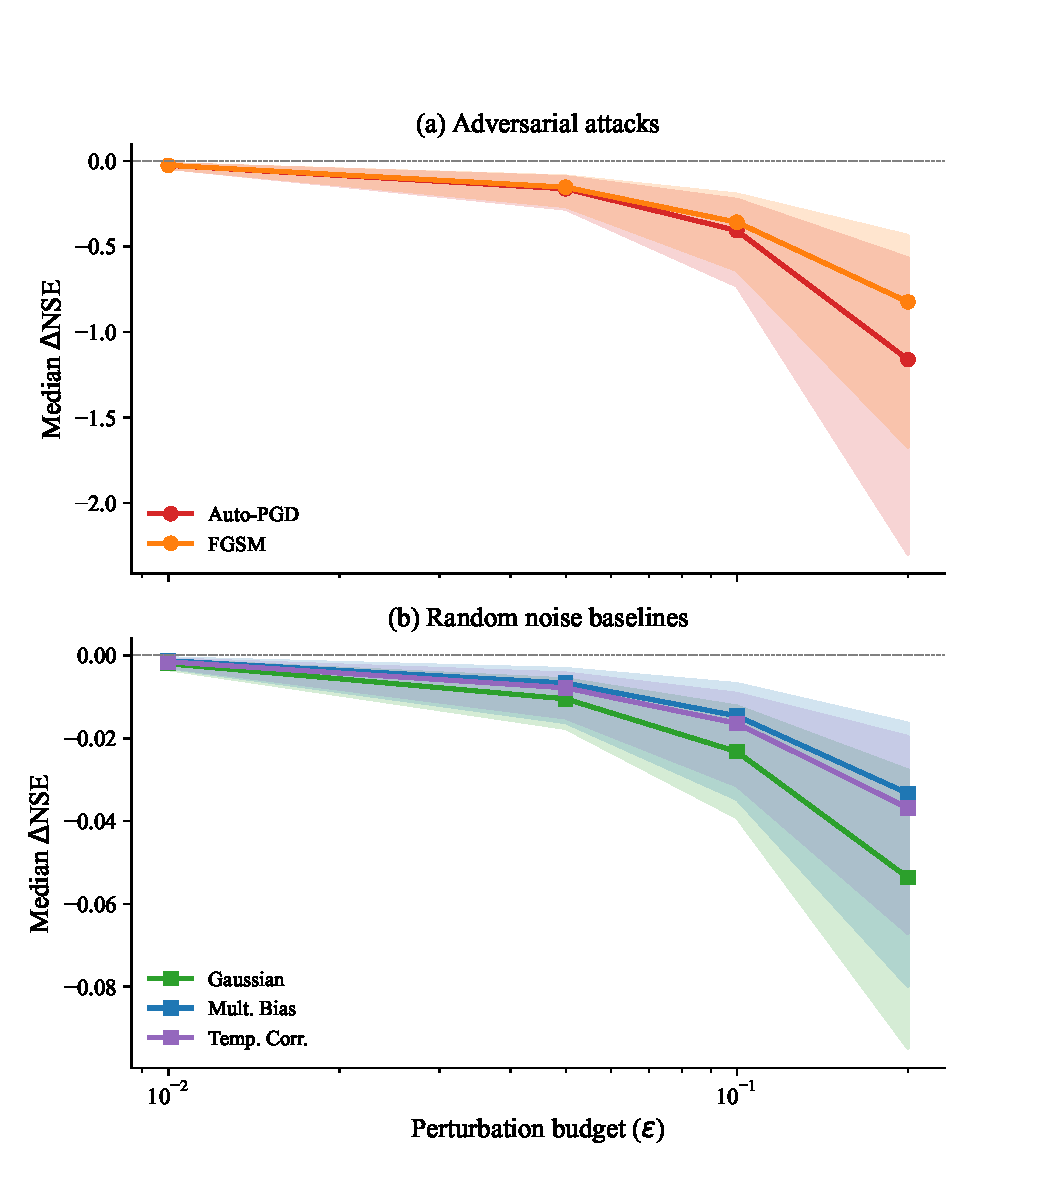
\includegraphics[width=\textwidth]{figures/fig1_epsilon_curve.pdf}
\caption{Median $\Delta$NSE as a function of $\varepsilon$ for five perturbation methods, with IQR shown as shaded bands. (a)~Adversarial attacks: Auto-PGD and FGSM. (b)~Random noise baselines. Note the different $y$-axis scales between panels.}
\label{fig:epsilon}
\end{figure}

At $\varepsilon = 0.1$, the median $\Delta$NSE under Auto-PGD is $-0.408$, compared to $-0.358$ for FGSM and $-0.023$ for Gaussian noise. All three random baselines cluster within a narrow band around $-0.02$ regardless of their temporal structure (Gaussian $-0.023$, multiplicative bias $-0.015$, temporally correlated noise $-0.016$), confirming that the dominant factor distinguishing methods is the use of gradient information rather than the temporal correlation of the perturbation. The Auto-PGD-to-Gaussian ratio at $\varepsilon = 0.1$ is 17.5$\times$, more than an order of magnitude larger than the Auto-PGD-to-FGSM ratio of 1.14$\times$.

The Auto-PGD-to-FGSM ratio grows monotonically with $\varepsilon$: 1.00$\times$ at $\varepsilon = 0.01$, 1.06$\times$ at $\varepsilon = 0.05$, 1.14$\times$ at $\varepsilon = 0.1$, and 1.41$\times$ at $\varepsilon = 0.2$ (Figure~\ref{fig:epsilon}). At small budgets the loss surface within the $\varepsilon$-ball is approximately linear, so a single gradient step nearly saturates the achievable damage; at larger budgets the local linear approximation breaks down and iterative refinement uncovers worse perturbations. The Auto-PGD-to-Gaussian ratio also grows with $\varepsilon$ (13.0$\times$, 15.6$\times$, 17.5$\times$, 21.6$\times$), so random-noise sensitivity analysis underestimates worst-case vulnerability most severely at the perturbation budgets that matter most for stress testing.

\subsubsection{Distribution-Level View at $\varepsilon = 0.1$}

Figure~\ref{fig:vulnerability} shows the per-basin distribution of $\Delta$NSE under Auto-PGD at $\varepsilon = 0.1$. The distribution is strongly right-skewed: the 10th percentile is $-1.51$, the median is $-0.408$, and the 90th percentile is $-0.12$. The distance between the 10th percentile and the median ($1.10$) is roughly 3.5 times the distance between the median and the 90th percentile ($0.29$), demonstrating that the median statistic alone hides a long tail of severely vulnerable basins.

\begin{figure}[ht]
\centering
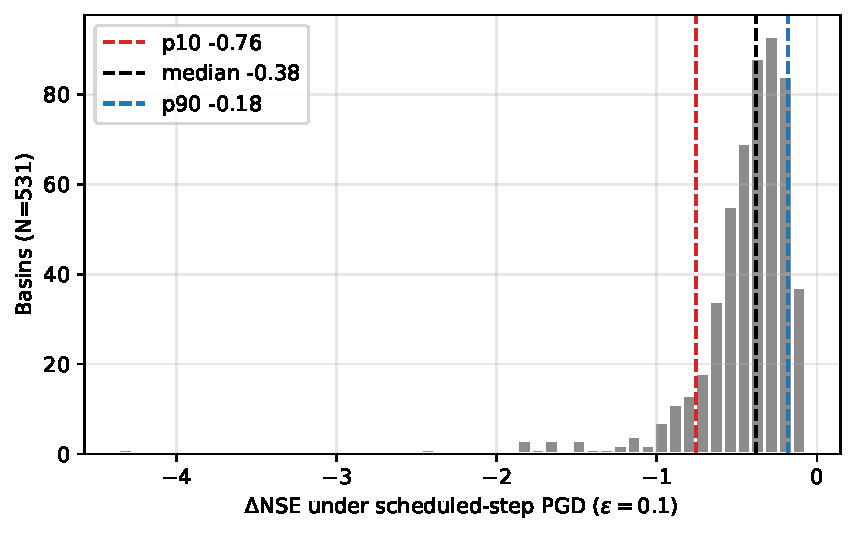
\includegraphics[width=\textwidth]{figures/fig2_basin_vulnerability.pdf}
\caption{Distribution of per-catchment $\Delta$NSE under Auto-PGD at $\varepsilon = 0.1$ ($N = 514$ finite NSE metrics from 531 basin IDs). Dashed lines mark the 10th percentile ($-1.51$), median ($-0.41$), and 90th percentile ($-0.12$).}
\label{fig:vulnerability}
\end{figure}

The size of this tail differs sharply across attack types. The fraction of basins with adversarial NSE below zero is 32.5\% under Auto-PGD, 28.8\% under FGSM, and 7.4\% under Gaussian noise. Under the stricter $\Delta$NSE $< -1$ threshold, Auto-PGD produces severe degradation in 90 of 514 finite basins (17.5\%). Even the cheapest gradient-based method (FGSM) identifies an at-risk population nearly four times larger than random noise, and iterative refinement adds another 3.7 percentage points of catchments below NSE $= 0$. Random-noise testing therefore underestimates not only the typical degradation but also the size of the at-risk tail population.

\subsection{Statistically Undetectable Perturbations Remain Effective}

Table~\ref{tab:constraint} presents the constraint-ablation results for Auto-PGD under three plausibility levels. Physical constraints (clipping precipitation to non-negative values and bounding temperatures to climatologically reasonable ranges) reduce median degradation by only 9\% relative to the $L_p$ baseline at $\varepsilon = 0.1$ (from $-0.408$ to $-0.370$), indicating that the most effective adversarial perturbations are often already physically plausible without explicit enforcement: the gradient direction does not require non-physical inputs to inflict near-worst-case damage.

Statistical constraints, which require the perturbed inputs to preserve the per-feature mean and standard deviation over the evaluation period, reduce median degradation by 53\% (to $-0.193$ at $\varepsilon = 0.1$). The reduction is larger than under physical constraints because preserving moments removes degrees of freedom along which the gradient most aggressively pushes the inputs, in particular the systematic shifts that bias the model's recurrent state.

\begin{table*}[ht]
\caption{Constraint ablation results for Auto-PGD (untargeted). Values are median (mean) $\Delta$NSE over the 514 finite basin metrics.}
\label{tab:constraint}
\centering
\small
\begin{tabular}{lrlll}
\toprule
Constraint & $N$ & $\varepsilon{=}0.05$ & $\varepsilon{=}0.1$ & $\varepsilon{=}0.2$ \\
\midrule
$L_p$ & 514 & $-$0.163 ($-$0.278) & $-$0.408 ($-$0.713) & $-$1.162 ($-$2.169) \\
Physical & 514 & $-$0.148 ($-$0.226) & $-$0.370 ($-$0.622) & $-$1.083 ($-$1.991) \\
Statistical & 514 & $-$0.083 ($-$0.113) & $-$0.193 ($-$0.258) & $-$0.459 ($-$0.633) \\
\bottomrule
\end{tabular}
\end{table*}

Crucially, the residual degradation under statistical constraints is operationally significant and grows with $\varepsilon$: from $-0.083$ at $\varepsilon = 0.05$ to $-0.193$ at $\varepsilon = 0.1$ to $-0.459$ at $\varepsilon = 0.2$. The ratio of statistical-constraint to $L_p$ degradation stays near $0.4$--$0.5$ across budgets, so moment-preserving perturbations recover roughly half of the unconstrained adversarial damage at every scale. The practical implication is direct: input data that passes standard quality-control checks by preserving feature-level means and standard deviations can still contain structured errors that substantially degrade model performance, and routine moment-based QC cannot rule out the existence of harmful input-error patterns within an observation-error-scale budget.

\subsection{Targeted Attacks and Pre-Event Vulnerability}

Table~\ref{tab:targeted} presents the results of targeted attacks. Flood-targeted attacks produce degradation comparable to, though slightly less than, untargeted attacks, while low-flow-targeted attacks are much weaker. The flood/low-flow contrast is approximately 16:1 by median $\Delta$NSE, indicating that vulnerability is concentrated in high-flow regimes.

\begin{table*}[ht]
\caption{Targeted attack results (Auto-PGD, $\varepsilon = 0.1$, $L_p$). Median [Q25, Q75] across finite basin metrics. $\Delta$NSE uses $N=514$; $\Delta$KGE uses all 531 basin IDs.}
\label{tab:targeted}
\centering
\small
\begin{tabular}{lrll}
\toprule
Target & $N$ & Median $\Delta$NSE [IQR] & Median $\Delta$KGE [IQR] \\
\midrule
Untargeted & 514 & $-$0.408 [$-$0.731, $-$0.225] & $-$0.380 [$-$0.819, $-$0.133] \\
Flood & 514 & $-$0.332 [$-$0.602, $-$0.182] & $-$0.344 [$-$0.716, $-$0.132] \\
Low-flow & 514 & $-$0.021 [$-$0.092, 0.003] & $-$0.049 [$-$0.236, 0.024] \\
\bottomrule
\end{tabular}
\end{table*}

Figure~\ref{fig:causal} shows the causal-trigger results. Restricting perturbations to progressively longer pre-event windows yields a monotonic increase in degradation: 1 day ($-0.011$), 3 days ($-0.028$), 7 days ($-0.050$), and 14 days ($-0.085$). Even perturbations confined to the 14 days preceding flood peaks cause non-trivial degradation concentrated in the operationally critical forecasting window.

\begin{figure}[ht]
\centering
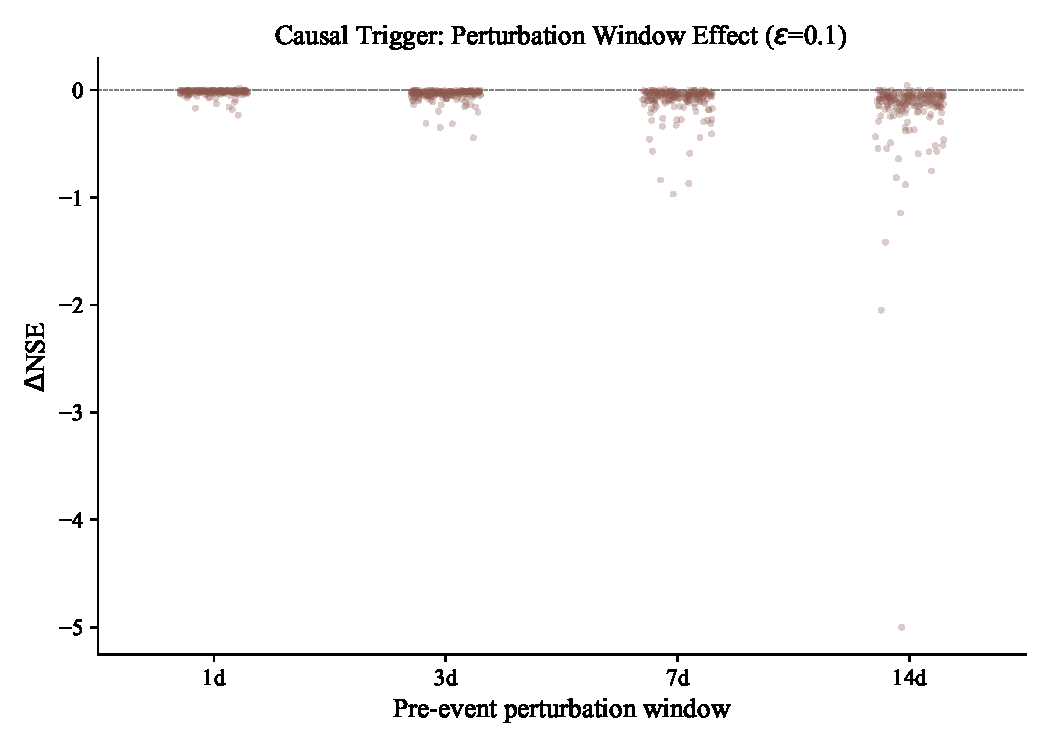
\includegraphics[width=\textwidth]{figures/fig3_causal_window.pdf}
\caption{Causal trigger: pre-event window length versus $\Delta$NSE ($\varepsilon = 0.1$). Box plots with jittered dots. Median values are annotated.}
\label{fig:causal}
\end{figure}

\subsection{Safety Margins and Detectability}

The previous subsections quantified how strongly the model can be degraded under fixed perturbation budgets. Two complementary questions characterize how silently this damage can occur: what is the minimum perturbation magnitude required to break the model, and can harmful perturbations be flagged by standard distribution tests on the input forcings? A small required perturbation that is also statistically invisible defines the worst case for input-side defenses.

The Carlini--Wagner (C\&W) attack identifies, for each basin, the minimum $L_2$ perturbation required to drive NSE below zero (Figure~\ref{fig:cw}). Of 531 basin IDs evaluated, 369 (69.5\%) yielded non-negligible solutions ($L_2 > 0.01$) with a median minimum perturbation of 1.244 in standardized units. The remaining 162 basins returned near-zero values, reflecting either an already low safety margin (the clean prediction is close to NSE $= 0$ to begin with) or failed convergence in the minimum-perturbation search rather than actual immunity. The median safety margin is on the same order as the standardized $\varepsilon = 1$ ball, but a non-trivial fraction of basins can be broken with $L_2 \ll 1$, particularly those with weaker baseline performance.

\begin{figure}[ht]
\centering
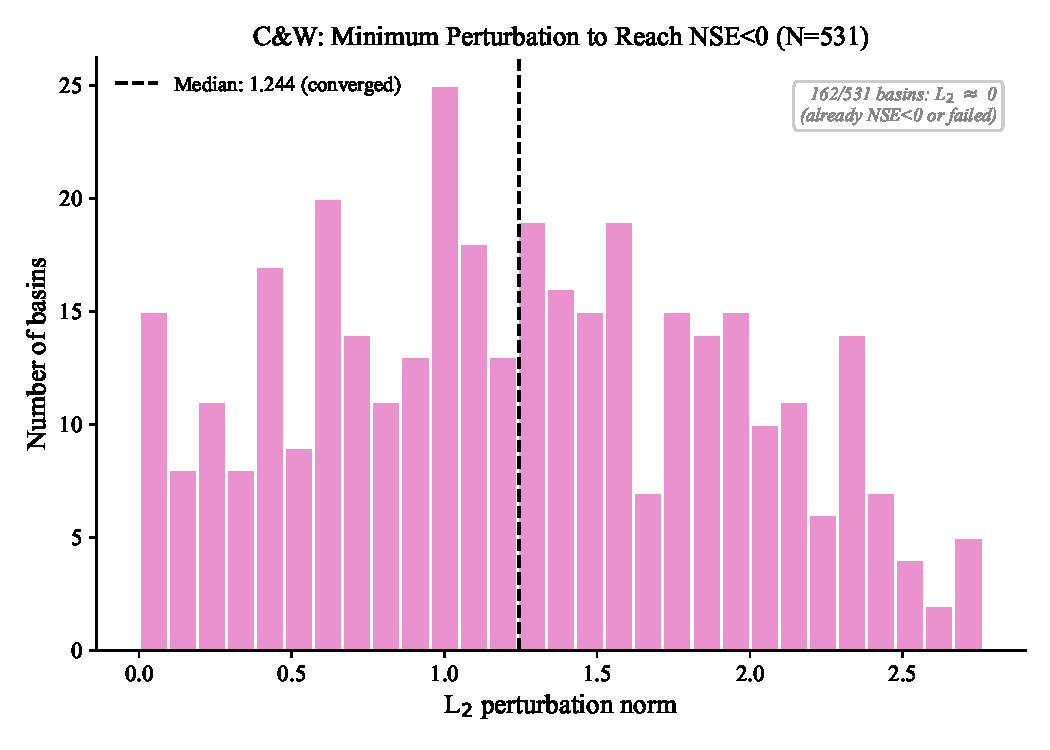
\includegraphics[width=0.8\textwidth]{figures/fig4_cw_perturbation.pdf}
\caption{Distribution of minimum $L_2$ perturbation required to reduce NSE below zero ($N = 531$ basin IDs). Non-negligible solutions use the analysis threshold $L_2 > 0.01$ ($N = 369$); 162 near-zero cases are annotated.}
\label{fig:cw}
\end{figure}

Detectability is assessed by computing a Kolmogorov--Smirnov (KS) two-sample test between the clean and perturbed input distributions for each forcing variable, and pairing the resulting $p$-value with the achieved $|\Delta\mathrm{NSE}|$. Figure~\ref{fig:detect} shows the joint distribution. Adversarial methods achieve large degradation across a wide range of $p$-values, including many cases with $p > 0.05$ that would not be flagged as statistically anomalous by a standard two-sample test. Effective adversarial perturbations therefore do not require statistical anomaly: they exploit the temporal-gradient structure of the model rather than violating the marginal input distributions, which is consistent with the constraint-ablation result that moment-preserving perturbations retain roughly half of the unconstrained damage.

\begin{figure}[ht]
\centering
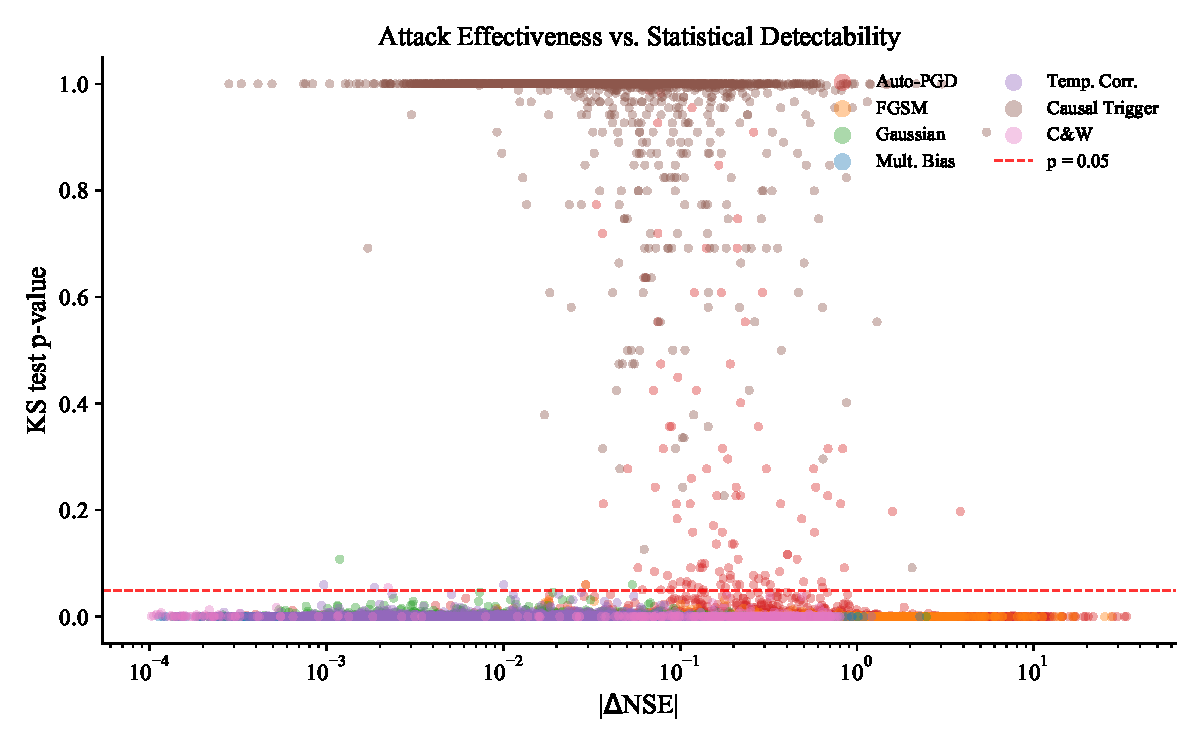
\includegraphics[width=\textwidth]{figures/fig5_detectability.pdf}
\caption{Attack effectiveness ($|\Delta\mathrm{NSE}|$) versus statistical detectability (KS $p$-value). The red dashed line marks $p = 0.05$.}
\label{fig:detect}
\end{figure}

Combining the two analyses, harmful perturbations exist whose $L_2$ magnitude is on the order of one standardized unit and whose marginal distributions remain statistically indistinguishable from the clean inputs. This is the worst case for input-side defenses based on summary-statistic monitoring and motivates the use of model-side detection or adversarial training rather than purely input-distribution checks.

%% ====================================================================
\section{Discussion}
%% ====================================================================

\subsection{Relation to Prior Adversarial Assessment of Hydrological LSTMs}

The closest precedent for this study is the FGSM-based robustness analysis of \citeA{Yang2026}, who applied single-step adversarial perturbations to LSTM and HBV rainfall-runoff models across 1{,}347 CAMELS-DE catchments. Their headline findings were that LSTMs were more robust than process-based HBV models, that catastrophic failure was rare, and that model responses scaled approximately linearly with perturbation magnitude. The 531-basin CAMELS-US results presented here qualify rather than contradict that picture.

At the same observation-error-scale budget ($\varepsilon = 0.1$), FGSM on our victim model produces a median $\Delta$NSE of $-0.358$ and pushes 28.8\% of finite basins below NSE $= 0$. Iterative Auto-PGD moves the median to $-0.408$ and the at-risk fraction to 32.5\%, with a further 17.5\% of basins falling below $\Delta$NSE $= -1$. Two of the three qualitative claims of \citeA{Yang2026} survive: random noise remains a much weaker probe than gradient-based attack, and the response to FGSM is approximately monotonic in $\varepsilon$ across our budget range. The third claim---that catastrophic failure is rare---is harder to defend once iterative methods and larger budgets are admitted, because severe degradation under Auto-PGD at $\varepsilon = 0.1$ is no longer a tail of curiosities but a population-level feature affecting roughly one in three finite basins.

The methodological complement is consistent with the broader adversarial machine-learning literature, in which single-step methods are documented to systematically overestimate model robustness \cite{Carlini2019}. The FGSM-to-Auto-PGD ratio observed here (1.14$\times$ at $\varepsilon = 0.1$, growing to 1.41$\times$ at $\varepsilon = 0.2$) transposes that pattern from image classification to a regression task on physical time series.

\subsection{Mechanisms Underlying the Attack-Method Hierarchy}

The hierarchy among the five methods at $\varepsilon = 0.1$---Auto-PGD followed by FGSM, with the three random baselines clustered near zero---admits a unified explanation. Random methods explore the input space isotropically and are exponentially unlikely to align with the directions of maximum sensitivity in the high-dimensional standardized input tensor. FGSM uses the local gradient at the clean input but takes a single step, so in regions where the loss surface has curvature within the $\varepsilon$-ball the sign of the clean-input gradient is not the direction of the worst attainable perturbation. Auto-PGD iteratively follows the surface, exploiting nonlinearities that FGSM cannot reach.

The adversarial-to-random gap (17.5$\times$ at $\varepsilon = 0.1$) far exceeds the FGSM-to-Auto-PGD gap (1.14$\times$), revealing the relative importance of the two methodological refinements: using gradient information at all matters far more than refining how that gradient is followed. The corresponding methodological recommendation is asymmetric: a single-step gradient-based attack should be a minimum requirement for any future hydrological robustness assessment, whereas iterative refinement is the natural gold standard for deployment-grade evaluations.

The constraint-ablation experiment provides a further mechanistic clue. Statistical constraints---which require the perturbed input to preserve per-feature mean and standard deviation---halve the median damage relative to the unconstrained $L_p$ baseline, but more than half of the damage remains. The residual damage therefore cannot be carried by changes in the marginal moments of the inputs; it must be carried by perturbations of temporal sequencing and cross-feature correlations to which the recurrent state is sensitive. Adversarial perturbations exploit the model's gradient structure rather than its absolute input scale, which explains why moment-based detectability tests (Section~3.4) cannot reliably flag them.

\subsection{Implications for Operational Hydrological Deployment}

These findings should not be read as evidence against the operational deployment of LSTM rainfall-runoff models. The adversarial perturbations are diagnostic rather than predictive: they test whether harmful error structures exist within observation-error-scale uncertainty budgets, not whether those exact perturbations are likely to occur in practice. A model that fails under such constrained stress tests cannot, however, be assumed robust on the basis of average-case random-noise experiments alone, because the stress test reveals harm that the random analysis is structurally unable to find.

A first implication concerns reporting conventions. Hydrological deep-learning studies routinely report clean-data NSE, KGE, and percentile error statistics across catchments. We suggest that an adversarial $\Delta$NSE at $\varepsilon = 0.1$ should accompany these summaries whenever a model is proposed for operational use. The marginal cost is modest---a single Auto-PGD pass per catchment over the test period---and the diagnostic power, as the Results above demonstrate, is qualitatively beyond what random-noise sensitivity analysis can provide.

A second implication concerns input quality control. Standard QC pipelines built around marginal-moment checks are well-suited to detecting gross sensor failure but are blind by construction to the moment-preserving perturbations isolated in the constraint-ablation experiment, even though such perturbations retain roughly half of the unconstrained adversarial damage at every budget tested. Detecting them would require higher-order input validation---temporal autocorrelation checks, cross-feature consistency tests, or model-side reconstruction residuals---rather than purely distributional checks at the feature-marginal level.

A third implication concerns the temporal structure of forecasting risk. The causal-trigger experiment shows that perturbations restricted to the fourteen days immediately preceding a flood peak still produce a median $\Delta$NSE of $-0.085$. In operational flood forecasting this is precisely the window in which input data are most consequential and most often degraded by sensor failure or telemetry latency. Robustness budgets and data-quality monitoring should therefore be tightened around such pre-event windows rather than applied uniformly across the entire time series.

\subsection{Caveats and Avenues for Future Work}

Several caveats bound the generality of these conclusions. The victim model is a single-layer LSTM with 128 hidden units and a fixed set of static catchment attributes; entity-aware LSTMs, sequence Transformers, and state-space architectures such as Mamba may interact with adversarial perturbations differently, and a systematic architectural sweep on the same 531-basin benchmark is the natural next step. The dataset is CAMELS-US at daily resolution; sub-daily datasets and non-CONUS hydroclimates, particularly those with stronger seasonal precipitation regimes, may shift both the median and the tail of the vulnerability distribution. Within the 531-basin benchmark itself, 17 basins yielded non-finite NSE-based robustness metrics because their evaluation windows lacked sufficient observed-flow variability for stable NSE calculation; headline statistics are therefore reported over the 514 finite basins while basin-coverage statements retain the full 531.

Defense strategies were intentionally outside the scope of this study. Adversarial training, ensemble averaging across model seeds, and input-side denoising each make a different methodological commitment, and a rigorous evaluation of these strategies---ideally against the same multi-level stress test rather than against FGSM alone---is a natural follow-up. The fact that statistically constrained perturbations retain about half of the unconstrained damage suggests that input-side denoising is unlikely to suffice on its own.

A final interpretive caveat is the diagnostic-not-predictive framing noted above. The adversarial perturbations here provide a worst-case bound within an observation-error-scale budget; they do not estimate the empirical frequency of such forcing-error patterns in operational settings. Closing that gap would require either coupling the attack to a calibrated input-error model or comparing the adversarial $\Delta$NSE distribution to the $\Delta$NSE distribution induced by historical input-error events. Both are open directions for future work.

%% ====================================================================
\section{Conclusions}
%% ====================================================================

We investigated how the choice of perturbation method affects adversarial robustness conclusions for a standard LSTM rainfall-runoff configuration, evaluating five methods spanning the spectrum from random noise to iterative gradient-based optimization across the 531-basin CAMELS-US temporal benchmark.

Our principal findings are:
\begin{enumerate}
\item \textbf{Attack-method choice has a decisive influence on robustness assessment.} Iterative adversarial perturbations reveal 17.5 times greater median vulnerability than Gaussian random noise at $\varepsilon = 0.1$; FGSM is closer but still weaker than Auto-PGD.
\item \textbf{Vulnerability is widespread under iterative attack.} At $\varepsilon = 0.1$, 167 of 514 finite basins (32.5\%) have adversarial NSE below zero under Auto-PGD.
\item \textbf{Statistically undetectable perturbations remain harmful.} Perturbations that preserve input-feature means and standard deviations still cause median $\Delta$NSE of $-0.193$ under Auto-PGD.
\item \textbf{Pre-event data quality is disproportionately important.} Perturbations restricted to the 14 days preceding flood peaks still cause median $\Delta$NSE of $-0.085$.
\end{enumerate}

Our results establish that robustness assessment for standard hydrological deep-learning configurations benefits from multi-level stress testing that goes beyond random noise and single-step adversarial methods. We recommend iterative adversarial evaluation at observation-error-scale budgets as a standard diagnostic component of hydrological stress-testing workflows, while broader architectural generalization remains future work.

\section*{Open Research}
All code for adversarial attacks, evaluation, and analysis is available at \url{https://github.com/[repository]}. The LSTM model was trained using the open-source neuralhydrology framework \cite{Kratzert2022}. CAMELS-US data are publicly available from the USGS \cite{Newman2015, Addor2017}.

\acknowledgments
[Acknowledgments to be added.]

\bibliography{references}

\end{document}
